\chapter{DISEÑO E IMPLEMENTACIÓN DEL CONJUNTO DE DATOS Y EL CLASIFICADOR DE COMENTARIOS OFENSIVOS EN BOLIVIA}\label{chp-resfttx}
La metodología utilizada en este proyecto se describió ampliamente en el capítulo 3, bajo el nombre de "canalización de Procesamiento de Lenguaje Natural (PLN)". Sin embargo, se consideró necesario añadir una fase de etiquetado de datos, ya que es especialmente relevante debido al uso del aprendizaje supervisado, que se seleccionó para los modelos propuestos. Asimismo, se eliminó la fase de monitoreo y actualización, ya que esta etapa se encuentra fuera del alcance de este proyecto. En la figura 5.1 se presenta la representación visual levemente modificada de la metodología de canalización de PLN seguida en este proyecto.

----------------------------

figura 5.1

-------------------------

Este enfoque permite optimizar continuamente el modelo para lograr la clasificación más precisa posible de comentarios en el contexto específico de redes sociales en Bolivia.

\section{DISEÑO}
Las tareas de limpieza, preprocesamiento de datos, etiquetado, manejo de archivos y formatos, y la creación e implementación de los modelos de clasificación se realizaron utilizando los siguientes módulos, los cuales se detallan a continuación:

\begin{itemize}
	\item	Preprocesamiento de comentarios: Este módulo fue creado para llevar a cabo cualquier tarea de preprocesamiento de texto necesaria para los datos adquiridos, así como para el manejo de formatos y archivos.
	
	\item Etiquetado de comentarios: Este módulo se desarrolló para realizar el etiquetado de todos los comentarios recolectados y preprocesados, preparándolos para su uso en el modelo.

	\item Creación y entrenamiento de modelos: En este módulo se diseñaron y ajustaron los diferentes modelos clasificadores de lenguaje ofensivo basados en redes neuronales convolucionales propuestos.
	
	\item Clasificador de lenguaje ofensivo en el contexto boliviano: Para utilizar el modelo clasificador, se creó una aplicación de escritorio que carga el modelo generado y permite la entrada de texto para clasificarlo en una de las tres clases propuestas.

\end{itemize}

Para visualizar de manera más detallada la infraestructura que permite la limpieza, preprocesamiento, construcción del conjunto de datos, creación y uso del modelo clasificador de comentarios, se creó el diagrama de clases 5.1. En este diagrama se representa cada módulo y su interacción.	

-------------------------------------------
Diagrama de clases 5.1

-----------------------------------------
\subsection{Preprocesamiento de comentarios}
En este módulo se detalla la implementación de cada paso del preprocesamiento de los datos, también conocido como canalización del procesamiento de lenguaje natural. Este proceso comienza con la adquisición de los datos, detallada en el capítulo 3, que consiste en numerosos documentos de texto que deben ser tratados.


El preprocesamiento de texto incluye diversas tareas de limpieza necesarias para los archivos de comentarios adquiridos, así como la corrección de lenguaje requerida y la conversión y tratamiento de formatos de los archivos. Esto asegura su limpieza y utilidad para el entrenamiento de modelos y el manejo de numerosos archivos. El resultado es un conjunto de datos útil, limpio, bien distribuido y en uno de los formatos estándar aceptables para el entrenamiento de los modelos propuestos.


Dado que las tareas son numerosas, el módulo se dividió en secciones, cada una con un propósito específico, las cuales se describen a continuación:

Limpieza de Datos

La carpeta limpiezadataset almacena los siguientes archivos:


\begin{itemize}

\item limpiar\_datos.py: Este archivo se encarga de los aspectos específicos de limpieza para cada fuente de información. Por ejemplo, la limpieza de datos extraídos de la red social Facebook no será la misma que la de datos provenientes de la red social WhatsApp. Las funciones y detalles de este archivo se ilustran en la figura \ref{fig:uml1}.

\begin{figure}
	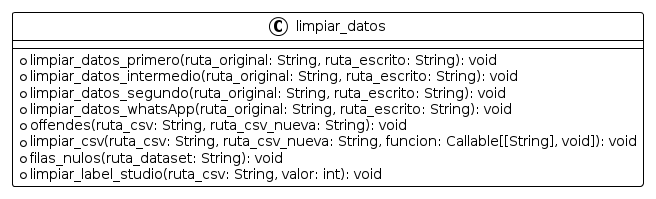
\includegraphics[width=0.65\textwidth]{capitulo5/figuras/fig1.png}
	\caption{Clase limpiar\_datos}
	\floatfoot{Fuente: Elaboración propia, generado con PlantUML}
	\label{fig:uml1}
\end{figure}

\item corrector\_lenguaje.py: Este archivo aborda los aspectos generales de limpieza que se aplican a cualquier tipo de información, independientemente de su fuente. Los detalles de este archivo se muestran en la figura \ref{fig:uml2}.

\begin{figure}
	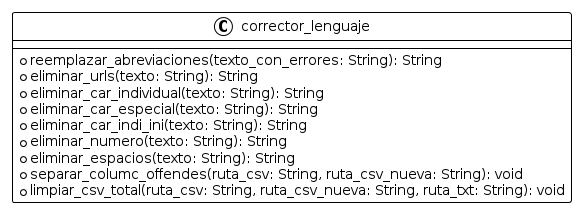
\includegraphics[width=0.65\textwidth]{capitulo5/figuras/fig2.png}
	\caption{Clase corrector\_lenguaje}
	\floatfoot{Fuente: Elaboración propia, generado con PlantUML}
	\label{fig:uml2}
\end{figure}

\end{itemize}

Formato y Encadenamiento de Información

La carpeta gestionarchivos contiene los siguientes archivos:

\begin{itemize}

\item manejo\_archivos.py: Este archivo se encarga de la creación, copia, recorrido y vaciado de archivos en diferentes formatos. Para más detalles, consulte la figura \ref{fig:uml3}.

\begin{figure}
	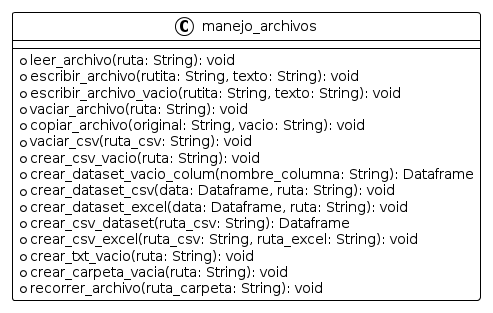
\includegraphics[width=0.65\textwidth]{capitulo5/figuras/fig3.png}
	\caption{Clase manejo\_archivos}
	\floatfoot{Fuente: Elaboración propia, generado con PlantUML}
	\label{fig:uml3}
\end{figure}


\item convertir\_formato.py: Este archivo se ocupa de agrupar información de múltiples archivos para hacer uso de forma masiva de las funciones de limpieza definidas en el archivo limpiar\_datos.py, además de manejar el formato de los mismos cuando sea necesario . Para más detalles, consulte la figura \ref{fig:uml4}.

\begin{figure}
	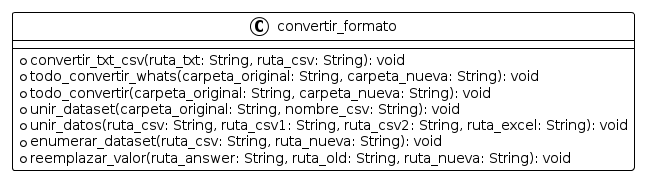
\includegraphics[width=0.65\textwidth]{capitulo5/figuras/fig4.png}
	\caption{Clase convertir\_formato}
	\floatfoot{Fuente: Elaboración propia, generado con PlantUML}
	\label{fig:uml4}
\end{figure}

\end{itemize}

Después de que los datos pasan por todo el proceso de canalización, se obtiene un producto final listo para ser utilizado en modelos de aprendizaje. Es importante recordar que el preprocesamiento de datos varía según la fuente de los datos. Para más detalles sobre el proceso de datos provenientes de Facebook, consulte la figura \ref{fig:um12} (diagrama de actividades de Facebook). El proceso de datos provenientes de WhatsApp se puede ver en la figura \ref{fig:um14}, y el proceso de limpieza del conjunto de datos ``offendes'' se detalla en la figura \ref{fig:um13}.

\begin{figure}
	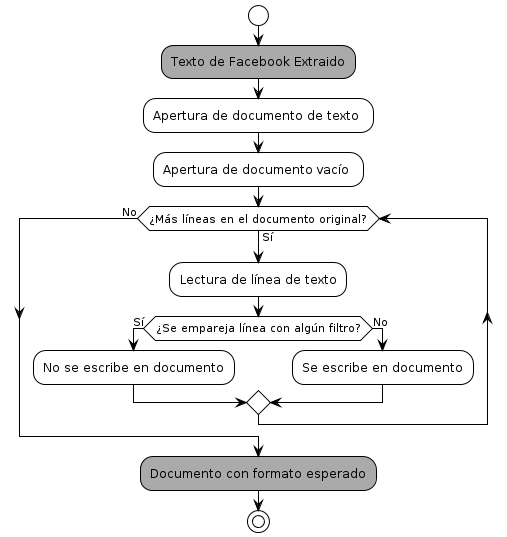
\includegraphics[width=0.65\textwidth]{capitulo5/figuras/part0.png}
	\caption{Diagrama de actividades limpieza datos facebook}
	\floatfoot{Fuente: Elaboración propia, generado con PlantUML}
	\label{fig:um12}
\end{figure}

\begin{figure}
	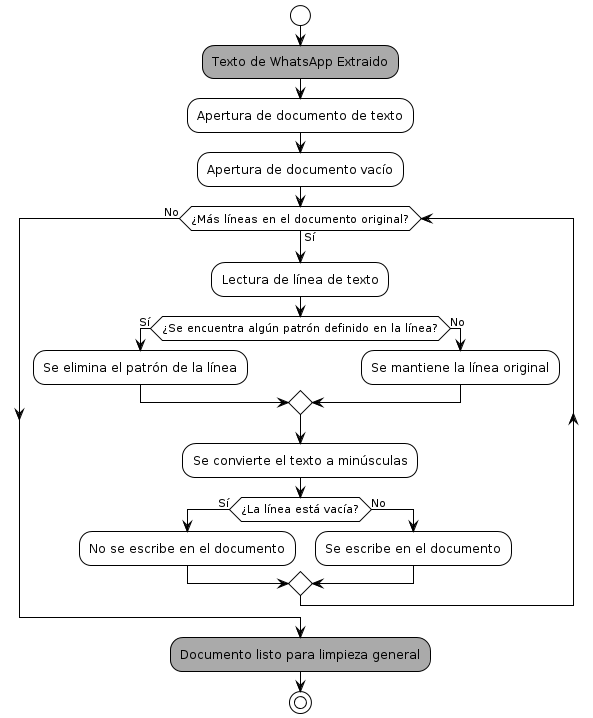
\includegraphics[width=0.65\textwidth]{capitulo5/figuras/part3.png}
	\caption{Diagrama de actividades limpieza datos whatsapp}
	\floatfoot{Fuente: Elaboración propia, generado con PlantUML}
	\label{fig:um14}
\end{figure}


\begin{figure}
	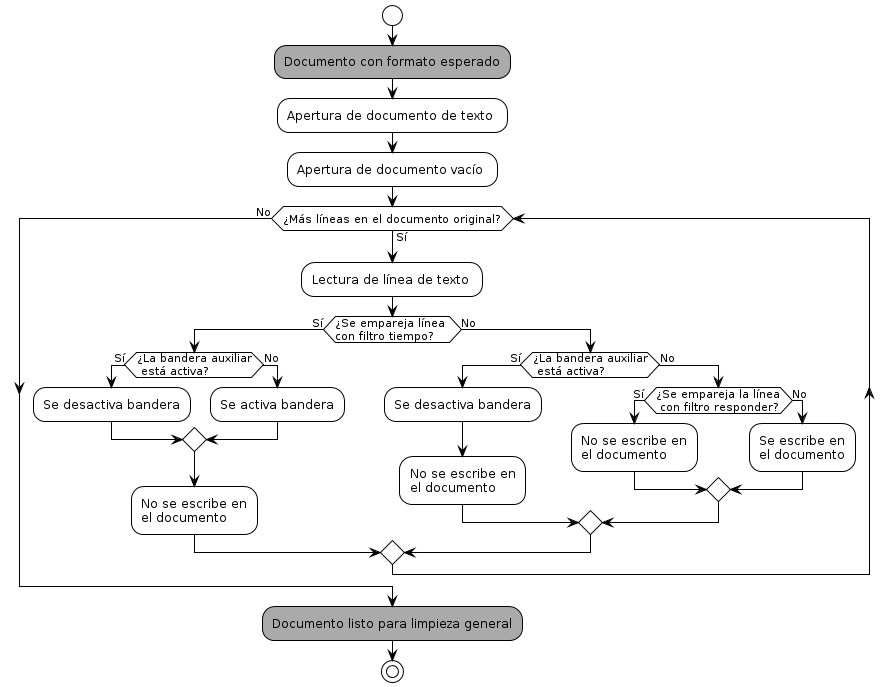
\includegraphics[width=0.65\textwidth]{capitulo5/figuras/part1.png}
	\caption{Diagrama de actividades  limpieza del conjunto de datos ``offendes''}
	\floatfoot{Fuente: Elaboración propia, generado con PlantUML}
	\label{fig:um13}
\end{figure}

\subsection{Etiquetado de comentarios}
En este módulo se incluyen todos los pasos necesarios para el etiquetado de los datos adquiridos con el modelo BERT, su revisión y reetiquetado. El mismo contiene las siguientes secciones:

Etiquetado de Comentarios

La carpeta etiquetadodatos almacena los siguientes archivos:

\begin{itemize}

\item operacion\_dataset.py: Este archivo se encarga de diversas operaciones necesarias para el entrenamiento del modelo BERT, como la mezcla de datos, el conteo de clases y la división de conjuntos de datos. Para más detalles, consulte la figura 5.

------------------------------------------

figura 5

-----------------------------------------

\item bert\_multi.py: Este archivo se ocupa de la creación, configuración, entrenamiento y predicción, entre otras tareas específicas del modelo BERT. Para más detalles, consulte la figura 6.

---------------------------------------

figura 6

--------------------------------------

\end{itemize}

Reetiquetado y Revisión de Etiquetas

Para el reetiquetado de los conjuntos de datos, se utilizó la herramienta Label Studio, que acepta archivos en varios formatos como CSV y TSV. Esta herramienta proporciona una interfaz cómoda que agiliza el proceso de revisión, etiquetado y reetiquetado. Además, ofrece filtros y otras funciones que permiten realizar cambios en cualquier conjunto de datos, los cuales pueden exportarse en distintos formatos.



\subsection{Creación y entrenamiento de modelos}
Este módulo abarca los procesos de distribución equilibrada de clases, visualización de secuencias, conteo de palabras y creación de la bolsa de palabras del conjunto de datos final. Además, se encarga del manejo de embeddings y de la creación, entrenamiento y evaluación de los modelos de redes convolucionales. Este módulo contiene las siguientes secciones:

Entrenamiento de Modelos

La carpeta entrenarmodelos almacena los siguientes archivos:

\begin{itemize}

\item creando\_dataset.py: Se encarga de la división de los conjuntos de datos en subconjuntos para el entrenamiento, la validación y la prueba, asegurando que cada una de las tres clases esté representada de la mejor manera para el entrenamiento de los modelos. También permite la visualización del estado del conjunto de datos, como el tamaño de secuencias y la bolsa de palabras. Ver figura 7.

------------------------------------------------
figura 7

--------------------------------------------------

\item preparar\_datos.py: Recibe el conjunto de datos en formato .CSV mismo que contiene comentarios textuales y sus etiquetas correspondientes. Convierte estos datos a listas para realizar procesos de tokenización, padding, carga de embeddings y procesamiento de embeddings, después de establecer los hiperparametros necesarios como el tamaño máximo de secuencia, el número máximo de palabras y la dimensión de los embeddings, además se crean métodos para el armado de la capa de embedding, compilación, entrenamiento, evaluación y graficación de los modelos Ver figura 8.

----------------------------------------------

figura 8

----------------------------------------------

\item cnn\_tres.py: Crea los modelos de redes convolucionales propuestos con una arquitectura base de tres capas. Ver figura 9.

---------------------------------------------

figura 9

---------------------------------------------

\item cnn\_four.py: Crea los modelos de redes convolucionales propuestos con una arquitectura base de cuatro capas. Ver figura 10.

------------------------------------------

figura 10

------------------------------------------

\item cnn\_dos.py: Crea los modelos de redes convolucionales propuestos con una arquitectura base de dos capas. Ver figura 11.

----------------------------------------

figura 11

---------------------------------------
\end{itemize}

Para la carga de embeddings, se utilizó la versión paga de Colab, debido a la necesidad de usar una mayor capacidad de memoria RAM. Las dimensiones de las estructuras utilizadas para la entrada y salida de las capas de embedding, capas de convolución, capas de max-pooling, etc., se detallarán más adelante.

Para cada modelo propuesto, se guarda una copia en cualquier época durante el entrenamiento en la que la pérdida del conjunto de validación disminuya. Además, para mayor comodidad, se almacena todo el historial de entrenamiento de cada modelo, permitiendo visualizar su avance y realizar comparaciones con otros modelos.

\subsection{Clasificador de lenguaje ofensivo en el contexto boliviano}
\input{capitulo5/clasificador}
\section{IMPLEMENTACIÓN}
La implementación de los módulos diseñados y detallados anteriormente se llevó a cabo en dos computadoras personales y un servicio en la nube con las siguientes características:

Computadora Personal 1

\begin{itemize}

\item Procesador: Intel Core i7 no especificado
\item Memoria RAM: no especificada
\item Sistema Operativo: Windows 10
\item Tarjeta Gráfica: No especificada

\end{itemize}

Computadora Personal 2

\begin{itemize}

\item Procesador: MacBook Pro (modelo específico no indicado)
\item Memoria RAM: No especificada
\item Sistema Operativo: macOS Monterey
\item Tarjeta Gráfica: No especificada

\end{itemize}

Servicio en la Nube

\begin{itemize}

\item Recurso de Hardware: Acceso a GPUs y TPUs de alta calidad (T4, A100, L4 y TPU v2)
\item Memoria RAM: Amplia capacidad
\item Tiempo de Ejecución: Prolongado, mayor a 12 horas de ejecución
\item Sistema Operativo: Linux personalizado

\end{itemize}

En las siguientes subsecciones se detallan las herramientas de software utilizadas y la implementación llevada a cabo para la clasificación de comentarios, etiquetado de comentarios, creación, entrenamiento y uso de los modelos generados en el proceso de prueba.

\subsection{Herramientas de Software}
El lenguaje de programación utilizado es Python, elegido por su sintaxis clara y fácil de leer, lo que permite centrarse más en la lógica del código y menos en los detalles sintácticos. Además, Python cuenta con una amplia variedad de bibliotecas y frameworks específicos para el aprendizaje automático y análisis de datos, tales como TensorFlow, Keras, PyTorch, Scikit-learn, Matplotlib, Seaborn y Pandas. Todas estas herramientas ofrecen funciones avanzadas que facilitan el desarrollo de proyectos en esta área, asi como BERT. El mismo es el modelo utilizado para el etiquetado de texto, y significa Bidirectional Encoder Representations from Transformers. Es un modelo de lenguaje preentrenado desarrollado por Google, tiene una arquitectura compuesta por múltiples capas de transformers, que son unidades básicas que procesan secuencias de entrada de manera bidireccional. Esto significa que el modelo puede capturar el contexto de una palabra en una oración teniendo en cuenta tanto las palabras que la preceden como las que la siguen, lo que lo hace extremadamente efectivo para una amplia gama de tareas de procesamiento del lenguaje natural. Esto se logra mediante el entrenamiento del modelo en dos tareas: 

\begin{itemize}
\item El modelado de lenguaje enmascarado (Masked Language Modeling, MLM) que ocurre durante el entrenamiento, donde BERT recibe una secuencia de palabras de entrada y algunas de estas palabras son enmascaradas aleatoriamente. La tarea del modelo es predecir qué palabra falta en cada lugar enmascarado, lo que obliga al modelo a comprender el contexto de las palabras en una oración para poder predecir la palabra enmascarada con precisión. Ver figura \ref{fig:nlp8}

\item Predicción de la siguiente oración: Además del MLM, BERT también se entrena en una tarea de predicción de la siguiente oración. Se le proporcionan dos oraciones y el modelo debe predecir si la segunda oración sigue a la primera en un contexto coherente o no.
\end{itemize}

\begin{figure}[h!]
	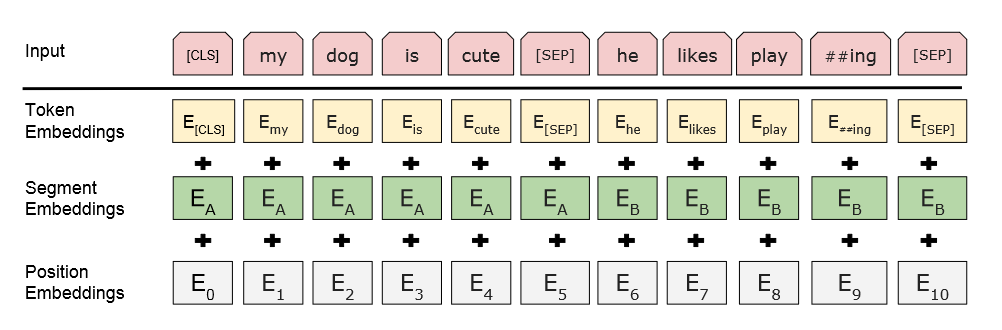
\includegraphics[width=0.65\textwidth]{capitulo3/figuras/nlp8.png}
	\caption[Representacion de entradas en BERT.]{Representacion de entradas en BERT.
		\\\textit{Fuente: Extraído de} \protect\cite[p. 5]{devlin2018bert} }
	\label{fig:nlp8}
\end{figure}

Para este proyecto, se utilizó la versión específica de BERT denominada ``bert\_uncased\_L-4\_H-512\_A-8'', una de las 24 variantes del conjunto ``BERT miniatura''. Estos modelos son versiones más compactas del BERT original, con una arquitectura reducida en comparación con BERT base o BERT grande, como se muestra en la tabla \ref{tbl:1}. Esto significa que tienen menos parámetros y requieren menos recursos computacionales para su entrenamiento y ejecución. Dado que los recursos necesarios para trabajar con un BERT base no están disponibles para este proyecto, utilizar este modelo compacto resultó extremadamente útil.

El modelo ``bert\_uncased\_L-4\_H-512\_A-8'' se entrena con texto en minúsculas, de ahí su denominación ``uncased''. Cuenta con cuatro capas (indicadas por ``L-4''), una dimensión de representación oculta de 512 en cada capa (indicada por ``H-512'') y utiliza ocho cabezas de atención en la capa de atención multi-cabeza (representadas por ``A-8'').

\begin{table}[!ht]
	\centering
	\caption[Representacion de versiones de BERT]{Representacion de versiones de BERT
		\\\textit{Fuente: Elaboracion Propia}}
	\begin{tabular}{|c|>{\centering\arraybackslash}m{2.5cm}|>{\centering\arraybackslash}m{2.5cm}|>{\centering\arraybackslash}m{3cm}|>{\centering\arraybackslash}m{2.5cm}|}
		\hline
		\textbf{} & \textbf{H=128} & \textbf{H=256} & \textbf{H=512} & \textbf{H=768} \\ \hline
		\textbf{L=2} & \makecell{2/128 \\ (BERT-Tiny)} & 2/256 & 2/512 & 2/768 \\ \hline
		\textbf{L=4} & 4/128 & \makecell{4/256 \\ (BERT-Mini)} & \makecell{4/512 \\ (BERT-Small)} & 4/768 \\ \hline
		\textbf{L=6} & 6/128 & 6/256 & 6/512 & 6/768 \\ \hline
		\textbf{L=8} & 8/128 & 8/256 & \makecell{8/512\\(BERT-Medium)} & 8/768 \\ \hline
		\textbf{L=10} & 10/128 & 10/256 & 10/512 & 10/768 \\ \hline
		\textbf{L=12} & 12/128 & 12/256 & 12/512 & \makecell{12/768 \\ (BERT-Base)} \\ \hline
	\end{tabular}
	\label{tbl:1}
\end{table}


Para cada tarea que se desee realizar con BERT, es crucial seleccionar los mejores hiperparámetros de ajuste a partir de las siguiente tabla \ref{tbl:2}:

\begin{table}[!ht]
	\centering
	\begin{tabular}{|c|c|}
		\hline
		\textbf{Hiperparametros} & \textbf{Valores} \\ \hline
		Tamaños de lote & 8, 16, 32, 64, 128 \\ \hline
		Tasas de aprendizaje & 3e-4, 1e-4, 5e-5, 3e-5 \\ \hline
		Número de épocas &  1, 2, 3, 4, 5 \\ \hline
		Tipo de capa de preprocesamiento & Según el modelo a usar \\ \hline
	\end{tabular}
	\caption[Detalle de hiperparametros y sus valores en BERT]{Detalle de hiperparametros y sus valores en BERT
		\\\textit{Fuente: Elaboracion Propia}}
	\label{tbl:2}
\end{table}

En este proyecto, para la tarea de etiquetado de los conjuntos de datos, se optó por un modelo de preprocesamiento ya entrenado específicamente seleccionado. La configuración específica incluyó:

\begin{itemize}

\item Capa de preprocesamiento: Una capa codificadora entrenable que se actualiza durante el entrenamiento(en-uncased-preprocess-version-3).
\item Capa de abandono: Con una tasa de abandono del 10\%.
\item Capa densa: Con una función de activación softmax para la clasificación múltiple.
\item Tamaño de lote: 32, lo que significa que los datos se dividen en lotes más pequeños con ese tamaño.
\item Tasa de aprendizaje: 3e-5.
\item Optimizador: AdamW.
\item Número de épocas: 5.

\end{itemize}

Para evaluar el modelo, se obtuvieron la pérdida y la precisión del modelo en el conjunto de prueba.

El entrenamiento del modelo BERT, el proceso de etiquetado de datos y la creación y entrenamiento de modelos de redes convolucionales se llevaron a cabo utilizando Google Colab (abreviatura de Colaboratory), una plataforma en línea proporcionada por Google. Colab permite escribir y ejecutar código Python en un entorno de cuaderno basado en la nube de forma gratuita como se muestra en la figura \ref{fig:bertito}. Está diseñado para facilitar la colaboración en proyectos de ciencia de datos y aprendizaje automático, así como para el desarrollo y experimentación con código Python sin necesidad de configurar un entorno local.

Google Colab ofrece acceso gratuito a recursos de cómputo en la nube, incluidas unidades de procesamiento gráfico (GPU) y unidades de procesamiento tensorial (TPU). Estos recursos fueron utilizados para el etiquetado de los conjuntos de datos. Sin embargo, el uso gratuito de CPU, GPU y TPU tiene limitaciones. Estas limitaciones se hicieron evidentes al entrenar el modelo BERT con grandes cantidades de datos, ya que el proceso requería mucho más tiempo de entrenamiento y el entorno se desconectaba, dejando el entrenamiento incompleto. Para evitar este problema, se adquirió el paquete Colab Pro, el cual garantiza que el entorno de ejecución no se desconecte y permite que BERT complete su entrenamiento sin interrupciones.

\begin{figure}[h!]
	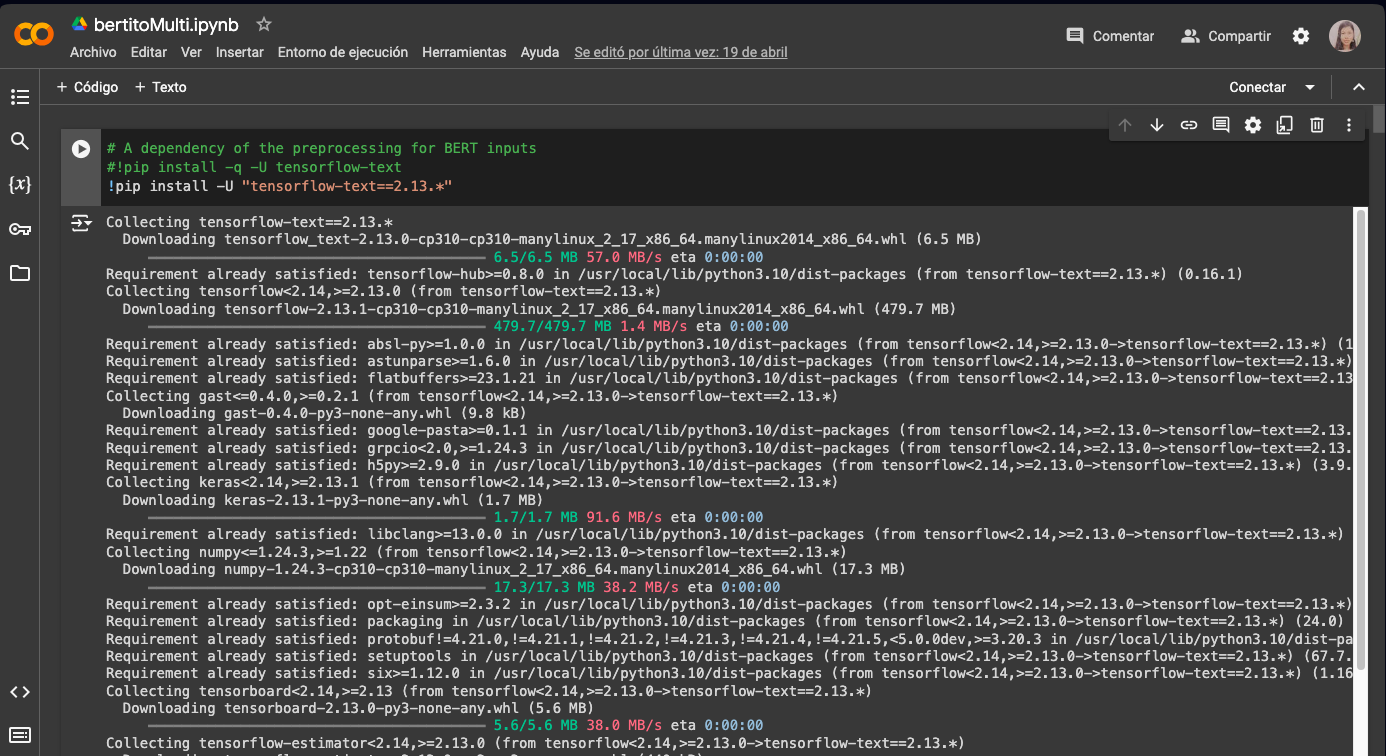
\includegraphics[width=1\textwidth]{capitulo5/figuras/bertito.png}
	\caption[Formato de cuaderno colab instalando libreria tensorflow-text-2.13]{Formato de cuaderno colab instalando libreria tensorflow-text-2.13
		\\\textit{Fuente: Elaboracion Propia}}
	\label{fig:bertito}
\end{figure}

Para la creación de los modelos de redes neuronales convolucionales se utilizó Keras, una API de alto nivel recomendada para TensorFlow a partir de su versión 1.14. Keras es una biblioteca de código abierto para la creación y entrenamiento de modelos de redes neuronales en Python. Es conocida por su facilidad de uso, ya que proporciona una interfaz de alto nivel que simplifica la construcción y el entrenamiento de modelos de redes neuronales. Los modelos de Keras se construyen utilizando capas que se pueden apilar o combinar de diversas formas para crear arquitecturas complejas.

A continuación, se detallan las versiones y bibliotecas utilizadas:

\begin{itemize}

\item Keras: 2.15.0
\item Matplotlib: 3.1.1
\item NumPy: 1.17.4
\item Python: 3.11.4
\item TensorFlow: 2.13.0 (para el modelo BERT)
\item Tensor-text: 2.13.0 (para el modelo BERT)
\item TensorFlow: 2.15.0 (para otros modelos)

\end{itemize}
\subsection{Preprocesamiento de comentarios}
A continuación, se presenta el código fuente de cada archivo de las secciones detalladas anteriormente en el módulo de preprocesamiento de comentarios:

Limpieza de Datos

En la sección de limpieza de datos se almacenan dos archivos. El código fuente \ref{lst:c1} corresponde al archivo limpiar\_datos.py, donde se puede observar la implementación de la limpieza de datos extraídos de las redes sociales, se usaron expresiones regulares en la implementación de cada función. 


\lstinputlisting[language=Python,firstline=7,caption=Codigo fuente limpieza de datos,label={lst:c1}]{capitulo5/codigo/limpiar_datos.py}


El código fuente \ref{lst:c2} corresponde al archivo corrector\_lenguaje.py, que se encarga de la limpieza general de un conjunto de datos. Esto incluye la eliminación de URLs, caracteres especiales, números, entre otros elementos, utilizando la biblioteca re de Python.

\lstinputlisting[language=Python,firstline=7,caption=Codigo fuente limpieza de URLs,label={lst:c2}]{capitulo5/codigo/corrector_lenguaje.py}

Formato y Encadenamiento de Información

La segunda y última sección de este módulo también almacena dos archivos y se enfoca en el tratamiento de archivos y formatos. En el código fuente \ref{lst:c3} se puede observar la implementación del archivo manejo\_archivos.py, que se encarga de crear, modificar, eliminar, y gestionar archivos en distintos formatos.

\lstinputlisting[language=Python,firstline=7,caption=Codigo fuente limpieza archivos y formatos,label={lst:c3}]{capitulo5/codigo/manejo_archivos.py}

En el código fuente \ref{lst:c4} se puede observar la implementación del último archivo de esta sección, convertir\_formato.py. Este archivo se encarga de recorrer múltiples archivos para compactar la información y realizar su conversión posterior. Además, se lleva a cabo el registro de cada archivo utilizado y de cada proceso realizado con ellos.

\lstinputlisting[language=Python,firstline=8,caption=Codigo fuente compactacion de informacion,label={lst:c4}]{capitulo5/codigo/convertir_formato.py}


\subsection{Etiquetado de comentarios}
A continuación, se presenta el código fuente de cada archivo de la sección detallada anteriormente en el módulo de etiquetado de comentarios:

Etiquetado de comentarios

En esta sección se almacenan dos archivos. El código fuente 1 corresponde al archivo bert\_multi.py, donde se puede observar la implementación del modelo Bert y cualquier función necesaria para el guardado de datos y del modelo mismo.

------------------------------------------

codigo fuente 1

-----------------------------------------

El código fuente 2 corresponde al archivo operacion\_dataset.py, que contiene las funciones implementadas para las operaciones necesarias en los conjuntos de datos utilizados por el modelo BERT.


----------------------------------------

codigo fuente 2

----------------------------------------
\subsection{Creación y entrenamiento de modelos}
Este módulo se divide en una sección con cinco archivos, encargada de todo el proceso necesario para entrenar los modelos de redes convolucionales.

Entrenamiento de modelos

A continuación se detalla cada archivo de la sección entrenamiento de modelos:

En el código fuente \ref{lst:c7} se puede observar la implementación del primer archivo, creando\_dataset.py, que visualiza el estado del conjunto de datos y lo divide manualmente, priorizando una distribución equilibrada entre las clases.

\lstinputlisting[language=Python,firstline=8,caption=Codigo fuente visualizacion estado del conjunto de datos,label={lst:c7}]{capitulo5/codigo/creando_dataset.py}

En el código fuente \ref{lst:c8} se observa la implementación del archivo preparar\_datos.py, que prepara la entrada final lista para la primera capa de los modelos propuestos. Esto implica la representación del texto en formas numéricas, en este caso, mediante embeddings. Además contiene funciones de armado, compilación, entrenamiento, entre otras funciones para los modelos de redes convolucionales

\lstinputlisting[language=Python,firstline=9,caption=Codigo fuente preparacion entrada final,label={lst:c8}]{capitulo5/codigo/preparar_datos.py}

En el código fuente \ref{lst:c9} se observa la implementación de todos los modelos de redes neuronales convolucionales basados en el modelo base propuesto, contenido en el archivo cnn\_tres.py.

\lstinputlisting[language=Python,firstline=7,caption=Codigo fuente  implementación de modelos de redes neuronales convolucionales,label={lst:c9}]{capitulo5/codigo/cnn_tres.py}

En el código fuente \ref{lst:c10} se observa la implementación de los modelos propuestos con diferentes arquitecturas a la arquitectura base para mejorar la precisión en la predicción de los otros modelos. Todo esto se encuentra en el archivo cnn\_cuatro.py.

\lstinputlisting[language=Python,firstline=7,caption=Codigo fuente implementación de los modelos con diferentes arquitecturas,label={lst:c10}]{capitulo5/codigo/cnn_cuatro.py}

Finalmente, en el código fuente \ref{lst:c11} se observa la implementación de todos los modelos de redes neuronales convolucionales con dos capas, contenido en el archivo cnn\_dos.py.

\lstinputlisting[language=Python,firstline=7,caption=Codigo fuente implementación de redes neuronales convolucionales con dos capas,label={lst:c11}]{capitulo5/codigo/cnn_dos.py}


\subsection{Clasificador de lenguaje ofensivo en el contexto boliviano}


\section{FLUJO DE TRABAJO}


\section{DESARROLLO DEL MODELO CLASIFICADOR}
Para establecer la arquitectura base, los hiperparámetros y cualquier configuración necesaria en los modelos base, se aprovechó principalmente la teoría detallada en este proyecto, así como la documentación expuesta de las herramientas en uso, donde se pueden observar los valores que pueden establecerse. Además, se tuvieron en cuenta trabajos relacionados o similares a la tarea en cuestión. Se optó por utilizar una red neuronal convolucional 1D debido a la naturaleza de los datos textuales. Los hiperparámetros específicos se detallarán más adelante.



\subsection{Hiperparámetros del modelo}
Los hiperparámetros utilizados se pueden dividir en dos categorías. En la primera se encuentran los hiperparámetros constantes, que no se modificaron durante ni después de las pruebas, esta sección se enfocara en estos hiperparámetros. Respecto a la segunda categoria donde se trata a los hiperparámetros que se modificaron durante las pruebas se detallarán al momento de describir los modelos y sus resultados.

En la tabla 5.1 se pueden observar los hiperparámetros utilizados para la capa de embedding en cada uno de los modelos convolucionales propuestos.

----------------------------------------

tabla 5.1

--------------------------------------

Para las capas restantes, como las capas de convolución, se detallan los hiperparámetros constantes en la tabla 5.2.

--------------------------------------

tabla 5.2

-------------------------------------



\subsection{Primera iteración}
Modelo Base

En la primera iteración de las pruebas, se utilizó una red convolucional 1D con tres capas de convolución, dos capas de maxpooling, una capa de globalmaxpooling y dos capas densas. Esta arquitectura se puede observar con más detalle en la figura 5.2. Los hiperparámetros base, como el numero de filtros, tamaño del stride, pool\_size, etc., se especifican en la tabla \ref{tbl:5}.

-----------------------------------------------------

figura 5.2

---------------------------------------------------

\begin{table}[!ht]
	\centering
	\begin{tabular}{|c|c|c|}
		\hline
		\textbf{Tipo de capa } & \textbf{Hiperparámetro } & \textbf{Valor} \\ \hline
		1ra capa convolucional 1D & num\_filtros, tam\_filtros, stride & 32, 3, 1 \\ \hline
		1ra capa maxpooling & tam\_pool, pool\_stride & 2, 2 \\ \hline
		2da capa convolucional 1D & num\_filtros, tam\_filtros, stride & 64, 5, 1 \\ \hline
		2da capa maxpooling & tam\_pool, pool\_stride & 2, 2 \\ \hline
		3ra capa convolucional 1D & num\_filtros, tam\_filtros, stride & 128, 5, 1 \\ \hline
		1ra capa densa intermedia & num\_neuronas & 128 \\ \hline
		2da capa densa de salida & num\_neuronas & 3 \\ \hline
	\end{tabular}
	\caption{Detalle arquitectura primera iteracion}
	\label{tbl:5}
\end{table}
  
En los resultados detallados en la figura algo1, se observa que el modelo sufre de sobreajuste. La precisión en el conjunto de entrenamiento aumenta constantemente a medida que avanzan las épocas, mientras que la precisión en el conjunto de validación disminuye. En la figura algo2, se muestra que el error en el conjunto de validación crece con el tiempo, mientras que el error en el conjunto de entrenamiento disminuye. Los resultados específicos se presentan en la tabla \ref{tbl:6}. Estos indicios sugieren la necesidad de utilizar técnicas de regularización para mitigar el sobreajuste.

---------------------------------------

figura algo 1

--------------------------------------

------------------------------------

figura algo 2

---------------------------------

\begin{table}[!ht]
	\centering
	\begin{tabular}{|c|c|c|c|c|c|}
		\hline
		\textbf{Nombre del modelo} & \textbf{Precisión} & \textbf{Perdida} & \textbf{Val\_Precisión} & \textbf{Val\_Perdida} & \textbf{Epoca} \\ \hline
		~ & 0.7522 & 0.59 & 0.7650 & 0.5743 & 3 \\ \cline{2-6} 
		cnn\_base\_tt & 0.978 & 0.04 & 0.7128 & 3.3866 & 109 \\ \cline{2-6} 
		~ & 0.9811 & 0.04 & 0.6893 & 3.8825 & 150 \\ \hline
	\end{tabular}
	\caption{Detalle resultados específicos primera iteracion}
	\label{tbl:6}
\end{table}

Modelo base y técnicas de regularización

A continuación, se detallan los modelos base utilizados junto con las técnicas de regularización aplicadas a cada uno. Se eligieron tres tipos de técnicas de regularización: normalización por lotes (batch normalization), regularización L2 y dropout. En esta iteración, se aplicó un tipo de regularización a cada capa convolucional. Los resultados obtenidos se presentan en la tabla \ref{tbl:7} y los detalles  sobre cada modelos a continuación:

\begin{itemize}
\item Modelo cnn\_base\_bn\_tt: Se aplicó normalización por lotes (batch normalization) a cada capa convolucional y a la capa densa intermedia.
\item Modelo cnn\_base\_dp\_tt: Se aplicó un dropout al 30\% a todas las capas convolucionales y un dropout al 50\% a la capa densa intermedia.
\item Modelo cnn\_base\_l2\_tt: Se aplicó regularización L2 con un valor de 0,05 a cada capa convolucional y a la capa densa intermedia.
\end{itemize}

\begin{table}[!ht]
	\centering
	\begin{tabular}{|c|c|c|c|c|c|}
		\hline
		\textbf{Nombre del modelo} & \textbf{Precisión} & \textbf{Perdida} & \textbf{Val\_Precisión} & \textbf{Val\_Perdida} & \textbf{Epoca} \\ \hline
		~ & 0.7890 & 0.52 & 0.7341 & 0.6090 & 4 \\ \cline{2-6} 
		cnn\_base\_bn\_tt & 0.9757 & 0.05 & 0.7272 & 2.8434 & 91 \\ \cline{2-6} 
		~ & 0.9800 & 0.04 & 0.5783 & 3.0617 & 150 \\ \hline
		~ & 0.7752 & 0.56 & 0.7646 & 0.5670 & 7 \\ \cline{2-6} 
		cnn\_base\_dp\_tt & 0.9000 & 0.25 & 0.7400 & 0.9013 & 133 \\ \cline{2-6} 
		~ & 0.9038 & 0.24 & 0.7274 & 0.8862 & 150 \\ \hline
		~ & 0.4185 & 1.02 & 0.4048 & 1.0484 & 123 \\ \cline{2-6} 
		cnn\_base\_l2\_tt & 0.4191 & 1.02 & 0.4048 & 1.0500 & 128 \\ \cline{2-6} 
		~ & 0.4118 & 1.02 & 0.4048 & 1.0503 & 150 \\ \hline
	\end{tabular}
	\caption{Detalle de los modelos base utilizados junto con las técnicas de regularización aplicadas}
	\label{tbl:7}
\end{table}

En los resultados detallados en la tabla \ref{tbl:7}, se observa que los métodos de regularización dropout y batch normalization (BN) retrasaron el sobreajuste. Sin embargo, al considerar el mejor modelo guardado con el menor error, el resultado es casi similar al obtenido por el modelo no regularizado. Por lo tanto, se probó el uso de dos técnicas de regularización simultáneamente en el modelo, manteniendo las mismas características pero modificando la capa densa intermedia a 64 y 32 neuronas en los modelos cnn\_base\_bndp\_64t y cnn\_base\_bndp\_32t, respectivamente. Los detalles y resultados se presentan en la tabla \ref{tbl:8}.

\begin{table}[!ht]
	\centering
	\begin{tabular}{|c|c|c|c|c|c|}
		\hline
		\textbf{Nombre del modelo} & \textbf{Precisión} & \textbf{Perdida} & \textbf{Val\_Precisión} & \textbf{Val\_Perdida} & \textbf{Epoca} \\ \hline
		~ & 0.8135 & 0.47 & 0.7596 & 0.5652 & 22 \\ \cline{2-6}
		cnn\_base\_bndp\_128t & 0.8967 & 0.26 & 0.7463 & 0.7757 & 126 \\ \cline{2-6}
		~ & 0.9029 & 0.25 & 0.7204 & 0.8861 & 150 \\ \hline
		~ & 0.7738 & 0.56 & 0.7777 & 0.5373 & 12 \\ \cline{2-6}
		cnn\_base\_bndp\_64t & 0.8701 & 0.34 & 0.7621 & 0.6211 & 65 \\ \cline{2-6}
		~ & 0.9058 & 0.25 & 0.7531 & 0.7155 & 150 \\ \hline
		~ & 0.8084 & 0.48 & 0.7804 & 0.5584 & 26 \\ \cline{2-6}
		cnn\_base\_bndp\_32t & 0.8580 & 0.37 & 0.7627 & 0.6342 & 56 \\ \cline{2-6}
		~ & 0.8962 & 0.28 & 0.7436 & 0.7562 & 150 \\ \hline
	\end{tabular}
	\caption{Detalle de los modelos base utilizados modificando la capa densa intermedia a 64 y 32 neuronas}
	\label{tbl:8}
\end{table}

Los resultados obtenidos en la tabla algo \ref{tbl;8} demuestran que, sin importar la época, el error en el conjunto de validación no sobrepasará 1.0 y siempre se mantendrá por debajo de ese rango. La precisión en el conjunto de validación se mantendrá siempre por encima de 0.75, siendo la mejor métrica de 0.78, obtenida por el modelo cnn\_base\_bndp\_32t, superando en 2 puntos la precisión del modelo base. Sin embargo, el modelo cnn\_base\_bndp\_64t fue el que obtuvo la menor pérdida.

\subsection{Segunda iteración}
En esta iteración se detallan los resultados obtenidos por los modelos con cuatro capas convolucionales, los detalles de la arquitectura base utilizada para cada modelo se especificaron anteriormente en la sección de modelado. 

Los resultados obtenidos en el modelo base, los modelos con una técnica de regularización y los modelos con dos técnicas de regularización se detallan en la tabla \ref{tbl:10}. Estos resultados no mostraron una mejora significativa en la precisión ni en la pérdida, por lo que se consideró innecesario desarrollar modelos más profundos. En su lugar, se decidió trabajar con un modelo menos profundo.


\begin{table}[!ht]
	\centering
	\begin{tabular}{|c|c|c|c|c|c|}
		\hline
		\textbf{Nombre del modelo} & \textbf{Precisión} & \textbf{Perdida} & \textbf{Val\_Precisión} & \textbf{Val\_Perdida} & \textbf{Epoca} \\ \hline
		~ & 0.7580 & 0.57 & 0.7714 & 0.5561 & 4 \\ \cline{2-6}
		cnn\_four & 0.8678 & 0.33 & 0.7206 & 0.8668 & 13 \\ \cline{2-6}
		~ & 0.9729 & 0.05 & 0.6937 & 4.4606 & 150 \\ \hline
		~ & 0.7870 & 0.53 & 0.7611 & 0.5810 & 11 \\ \cline{2-6}
		cnn\_dp\_four & 0.8528 & 0.37 & 0.7501 & 0.6475 & 41 \\ \cline{2-6}
		~ & 0.9019 & 0.25 & 0.7297 & 0.8340 & 150 \\ \hline
		~ & 0.8158 & 0.46 & 0.7650 & 0.5887 & 31 \\ \cline{2-6}
		cnn\_dp\_four\_f & 0.8665 & 0.35 & 0.7430 & 0.6575 & 108 \\ \cline{2-6}
		~ & 0.8726 & 0.33 & 0.7263 & 0.7339 & 150 \\ \hline
		~ & 0.8013 & 0.80 & 0.7699 & 0.5947 & 45 \\ \cline{2-6}
		cnn\_dp\_four\_fi & 0.8203 & 0.45 & 0.7625 & 0.6179 & 79 \\ \cline{2-6}
		~ & 0.8300 & 0.41 & 0.73 & 0.66 & 150 \\ \hline
		~ & 0.7611 & 0.59 & 0.7442 & 0.6174 & 19 \\ \cline{2-6}
		cnn\_bndp\_four\_f & 0.8096 & 0.48 & 0.7314 & 0.6467 & 42 \\ \cline{2-6}
		~ & 0.8662 & 0.34 & 0.5514 & 2.0138 & 150 \\ \hline
		~ & 0.7890 & 0.53 & 0.7650 & 0.5887 & 55 \\ \cline{2-6}
		cnn\_bndp\_four\_fi & 0.8021 & 0.49 & 0.7630 & 0.6190 & 74 \\ \cline{2-6}
		~ & 0.8345 & 0.41 & 0.7403 & 0.6992 & 150 \\ \hline
		~ & 0.7768 & 0.62 & 0.7255 & 0.5657 & 128 \\ \cline{2-6}
		cnn\_bndp\_four\_ss & 0.7849 & 0.54 & 0.7349 & 0.6329 & 141 \\ \cline{2-6}
		~ & 0.7832 & 0.54 & 0.7282 & 0.6471 & 150 \\ \hline
	\end{tabular}
	\caption{Detalle resultados obtenidos
		\\\textit{Fuente: Elaboracion Propia}}
	\label{tbl:10}
\end{table}

%\subsection{Tercera iteración}
%En esta sección se detallan los resultados del modelo base y  los modelos  base con una técnica de regularización con dos capas convolucionales, estos se muestran en  la tabla \ref{tbl:12}.

\begin{table}[!ht]
	\centering
	\begin{tabular}{|c|c|c|c|c|c|}
		\hline
		\textbf{Nombre del modelo} & \textbf{Precisión} & \textbf{Perdida} & \textbf{Val\_Precisión} & \textbf{Val\_Perdida} & \textbf{Epoca} \\ \hline
		cnn\_two & 0.7686 & 0.56 & 0.7787 & 0.5356 & 3 \\ \cline{2-6}
		~ & 0.9765 & 0.06 & 0.7004 & 2.2804 & 50 \\ \hline
		cnn\_dp\_two & 0.7747 & 0.55 & 0.7819 & 0.5524 & 8 \\ \cline{2-6}
		~ & 0.8718 & 0.32 & 0.7441 & 0.7408 & 50 \\ \hline
		cnn\_dp\_two1 & 0.7620 & 0.55 & 0.7746 & 0.5454 & 6 \\ \cline{2-6}
		~ & 0.9265 & 0.19 & 0.7303 & 1.0931 & 50 \\ \hline
	\end{tabular}
	\caption{Detalle resultados obtenidos}
	\label{tbl:12}
\end{table}




\subsection{Tercera iteración}
Como última iteración, se experimentó con una red menos profunda de dos capas. La red convolucional cnn\_two se estableció como la arquitectura base, sus hiperparámetros y estructura se describen en la tabla 5. A partir de esta arquitectura, se añadieron técnicas de regularización dropout en los modelos propuestos, cuyos resultados se detallan en la tabla algo 6.

\begin{itemize}

\item Al modelo cnn\_dp\_two se le aplicó un dropout del 30\% después de cada capa convolucional y un dropout del 50\% después de la capa densa intermedia.

\item Al modelo cnn\_dp\_two1 se le aplicó un dropout del 10\% después de cada capa convolucional y un dropout del 20\% después de la capa densa intermedia.


-------------------------------

tabla algo 5

----------------------------------


-----------------------

tabla algo6

----------------------------
\end{itemize}
\section{RESULTADOS}



